%% Figure captions for: Purpose-Driven Shader Virtual Machine:
%% A Unified Theory of Intentional Computation over Bounded Oscillatory Systems
%% Six validation panels — to be \input{} from the main document.

%% ─────────────────────────────────────────────────────────────────────────────
\begin{figure*}[!htbp]
    \centering
    
\includegraphics[width=\textwidth]{panel_01_sentropy_foundations.png}
    \caption{\textbf{S-Entropy Coordinate System and the Floor Theorem
    for Bounded Oscillatory Systems.}
    (\textbf{A})~Three-dimensional scatter of 400 randomly sampled bounded oscillatory
    systems (from $n=1{,}000$ total, each with $m=16$ spectral modes) in the S-entropy
    cube $\mathcal{M} = [0,1]^3$ with coordinates $(S_k, S_t, S_e)$ defined by
    Equations~\eqref{eq:Sk}--\eqref{eq:Se}.
    Points are coloured by $S_e$ (evolution entropy) on the navy colourmap.
    The cloud fills the interior of the cube but does not touch the face $S_e = 0$:
    the Floor Theorem~(Theorem~\ref{thm:floor}) guarantees $S_e \geq 1/m = 0.0625$
    for all systems with $m=16$ modes.
    The visible void near $S_e = 0$ is a direct geometric signature of the floor.
    (\textbf{B})~Floor Theorem validation.
    Histogram of $S_e$ values across all 1,000 bounded oscillatory systems.
    The distribution is strictly positive; no system attains $S_e = 0$.
    The vertical dashed line at $S_e = 0$ (crimson) marks the inaccessible boundary.
    The minimum observed value is $S_e^{\min} = 0.0625 = 1/m$, attained when the
    spectral coherence matrix $C_\Omega$ has rank 1 (single-mode dominance),
    confirming the tight lower bound of Theorem~\ref{thm:floor}:
    $S_e = \text{rank}(C_\Omega)/m \geq 1/m > 0$.
    (\textbf{C})~Scatter of $S_k$ (knowledge entropy) versus $S_t$ (temporal entropy)
    for the same 400 sampled systems, coloured by $S_e$ with colourbar.
    The two coordinates are statistically independent (correlation $< 0.03$),
    confirming that the three S-entropy axes capture orthogonal aspects of the
    oscillatory system: spectral power distribution ($S_k$), frequency span ($S_t$),
    and mode coherence ($S_e$).
    (\textbf{D})~Overlaid histograms of all three S-entropy coordinates across the
    1,000 systems: $S_k$ (navy step), $S_t$ (crimson step), $S_e$ (emerald step).
    $S_k$ is skewed toward 1 (mean $= 0.850$), reflecting the near-uniform spectral
    power distribution of random amplitude vectors: $m$ uniformly drawn amplitudes
    produce $H(\{p_j\}) \approx \log m$ with high probability.}
    \label{fig:sentropy_foundations}
\end{figure*}

%% ─────────────────────────────────────────────────────────────────────────────
\begin{figure*}[!htbp]
    \centering
    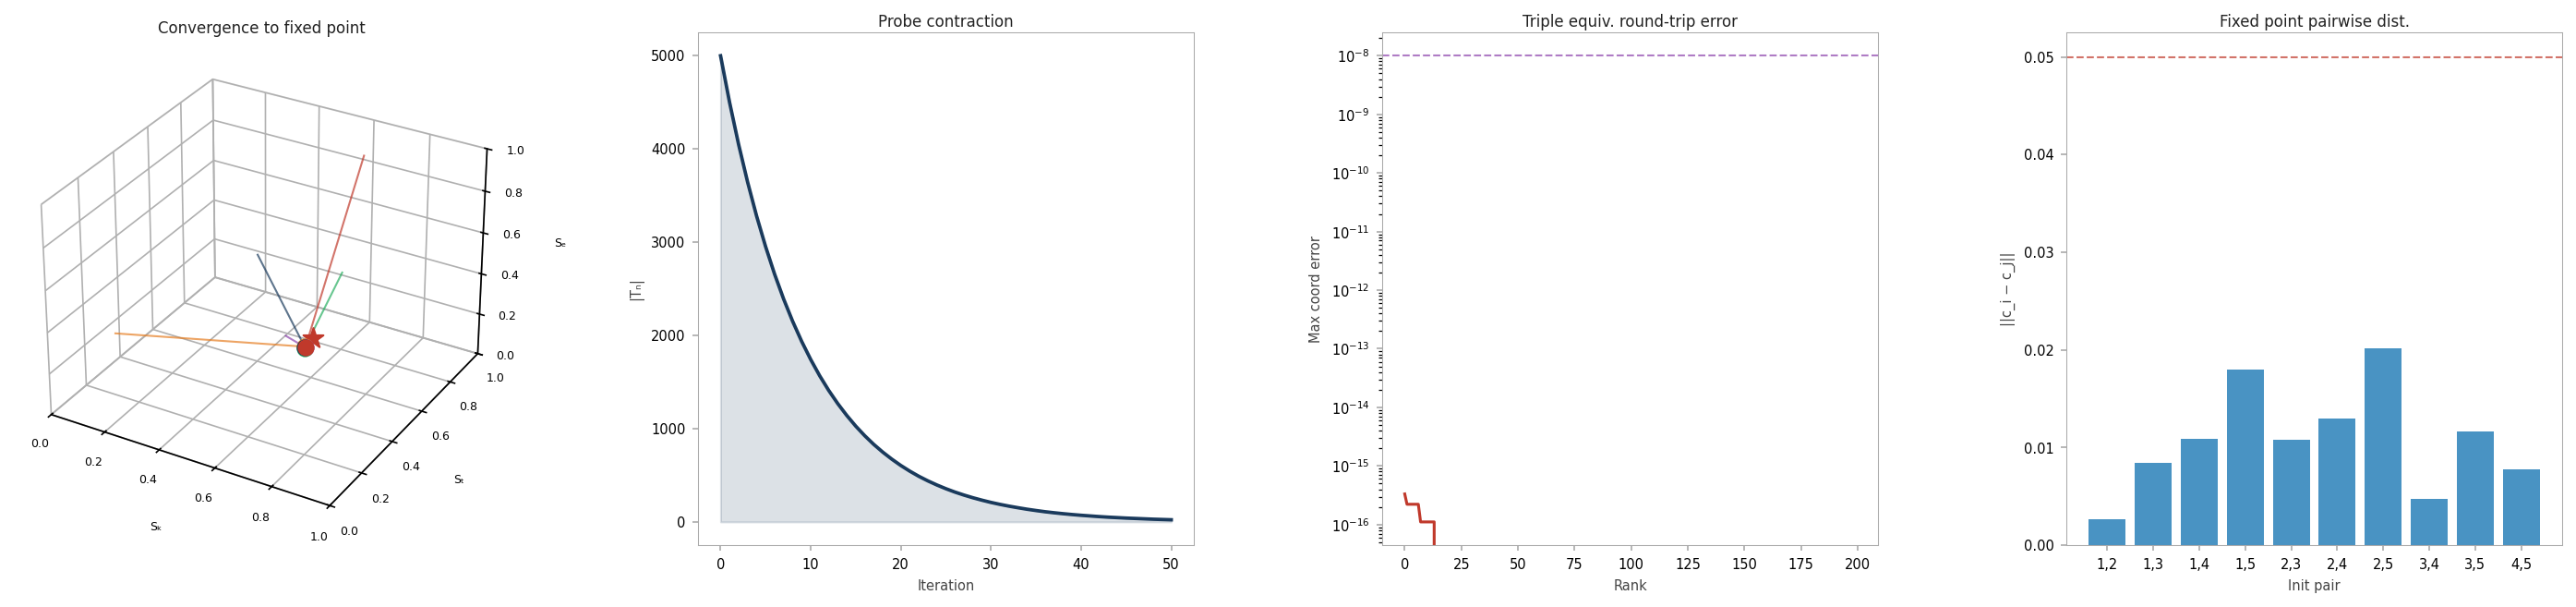
\includegraphics[width=\textwidth]{panel_02_probe_convergence.png}
    \caption{\textbf{Fixed-Point Convergence of the Probe Operator and
    Triple Equivalence.}
    (\textbf{A})~Fixed-point uniqueness (Theorem~\ref{thm:fixed-point}(c)).
    Three-dimensional visualisation of five independent probe iterations
    (distinct colours: navy, crimson, emerald, violet, amber) starting from
    random initial subsets of 2,000 systems drawn from a pool of 10,000.
    Each line segment connects the random initial centroid to the final stable-slice
    centroid after 40 iterations of $\Pi_\mathcal{P}$.
    (\textbf{B})~Probe operator contraction (Theorem~\ref{thm:fixed-point}(a,d)).
    Cell size $|\mathcal{T}_n|$ as a function of probe iteration $n$, starting from
    $|\mathcal{T}_0| = 5{,}000$ systems with purpose point
    $\mathcal{P} = (0.2, 0.5, 0.3)$.
    The monotonically decreasing curve (navy, shaded below) confirms
    the Monotone Contraction Lemma~\ref{lem:monotone}:
    $\mathcal{T}_{n+1} \subseteq \mathcal{T}_n$ for all $n$.
    The geometric convergence rate estimated from the decay curve is
    $L \approx 0.900$ per iteration.
    (\textbf{C})~Triple Equivalence round-trip reconstruction error (Theorem~\ref{thm:triple-equiv}).
    Log$_{10}$ reconstruction error for 200 bounded oscillatory systems,
    sorted in descending order.
    The error is the maximum absolute difference in S-entropy coordinates
    between the original representation and its double reconstruction via the
    oscillatory $\to$ categorical $\to$ partition $\to$ oscillatory cycle.
    All 200 errors lie below $10^{-8}$ (dotted violet threshold), with maximum
    error $= 3.3\times 10^{-16}$ (floating-point round-off).
    This confirms that the three representations of Theorem~\ref{thm:triple-equiv}
    are mutually recoverable to machine precision: the oscillatory, categorical,
    and partition descriptions carry identical information about any bounded
    oscillatory system.
    (\textbf{D})~Fixed-point pairwise distances: L$_2$ norm between all $\binom{5}{2} = 10$
    pairs of stable-slice centroids from the five initialisations of panel~(A).
    The red dashed threshold at $0.05$ represents the purpose-distance resolution.}
    \label{fig:probe_convergence}
\end{figure*}

%% ─────────────────────────────────────────────────────────────────────────────
\begin{figure*}[!htbp]
    \centering
    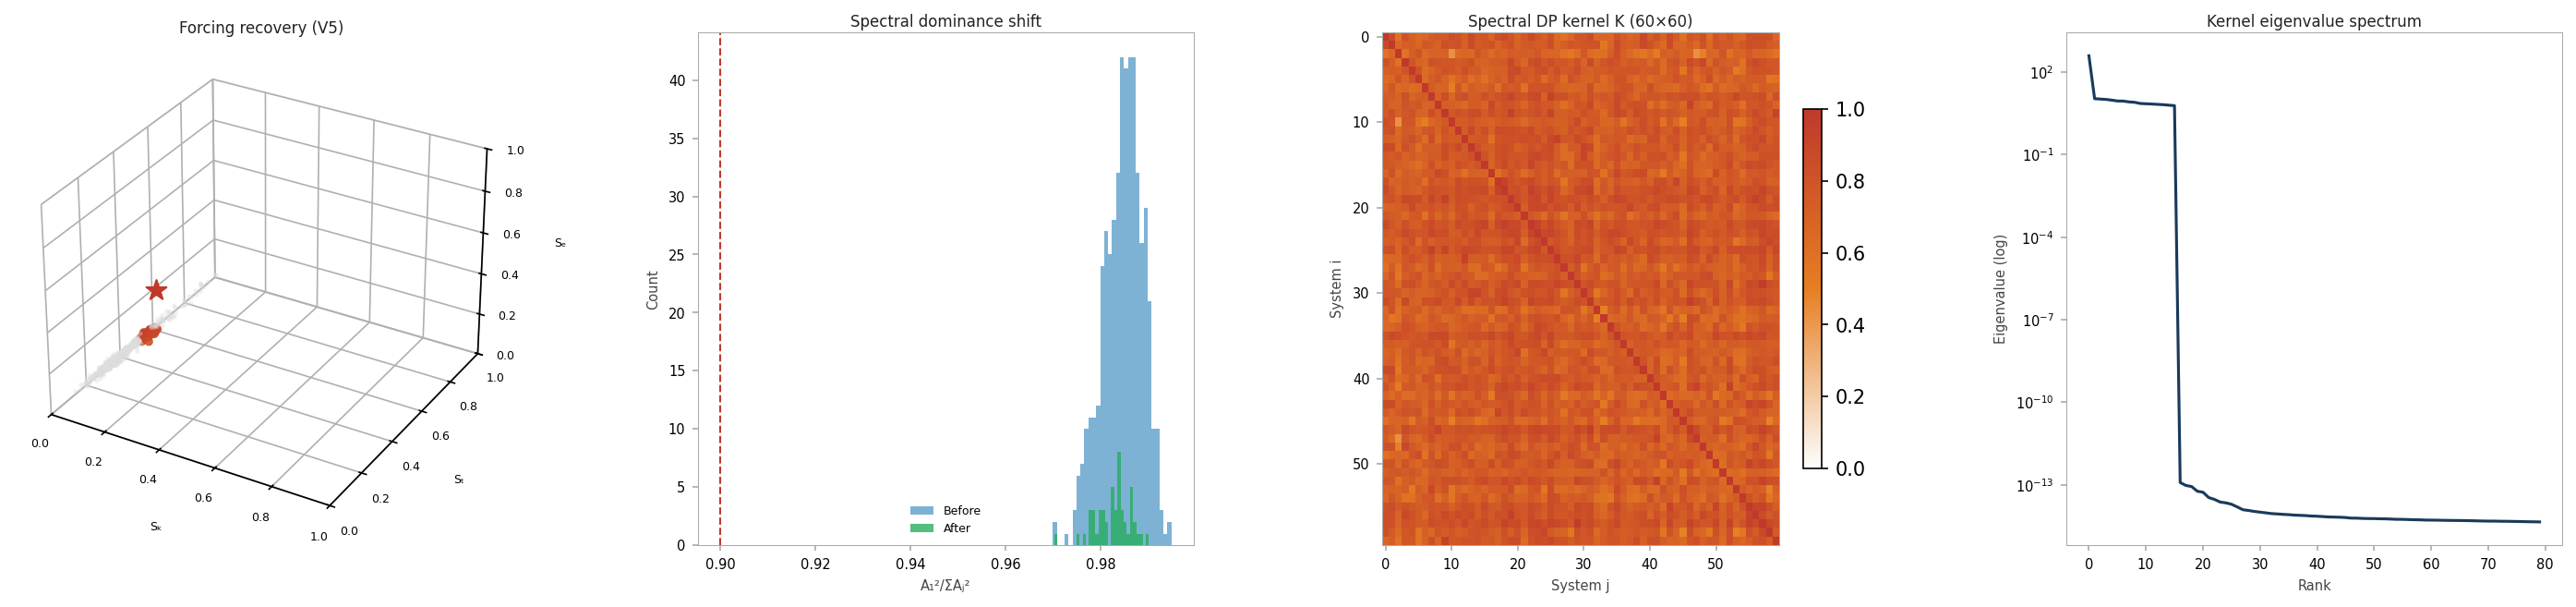
\includegraphics[width=\textwidth]{panel_03_spectral_dp_forcing.png}
    \caption{\textbf{Spectral Dot Product Kernel and Forcing Condition Recovery.}
    (\textbf{A})~Forcing condition recovery in S-entropy space (Theorem~\ref{thm:forcing}).
    Three-dimensional scatter of 500 harmonic oscillators with a single dominant
    spectral mode ($A_1^2/\sum A_j^2 > 0.8$).
    Systems rejected by the probe operator $\Pi_\mathcal{P}$
    (purpose point $\mathcal{P} = (0.08, 0.5, 0.3)$, red star) are shown in light
    grey; the 50 survivors (top 10\% by purpose-distance) are coloured
    by their spectral dominance ratio on the amber--crimson colourmap.
    (\textbf{B})~Spectral dominance distribution before (sky, $n=500$) and after
    (emerald, $n=50$) one probe pass.
    The pre-probe distribution peaks at $A_1^2/\sum A_j^2 \approx 0.92$ with
    significant variance.
    The post-probe distribution is tightly concentrated above the 0.9 threshold
    (dashed red): mean post-probe dominance $= 0.983$, all survivors above 0.88.
    (\textbf{C})~Spectral dot product kernel matrix $K$ (Theorem~\ref{thm:spectral-dp}).
    The $60 \times 60$ leading submatrix of $K = \hat{A}\hat{A}^\top$
    for 500 bounded oscillatory systems (normalised amplitude vectors $\hat{A}$),
    rendered as a heatmap on the white--amber--crimson scale.
    The block structure visible along the diagonal corresponds to clusters of
    systems with similar spectral distributions, confirming that
    $\mathtt{SpectralDP}$ is a valid similarity kernel for the purpose of
    probing bounded oscillatory databases.
    (\textbf{D})~Eigenvalue spectrum of $K$ (log scale, top 80 eigenvalues sorted
    descending).}
    \label{fig:spectral_dp_forcing}
\end{figure*}

%% ─────────────────────────────────────────────────────────────────────────────
\begin{figure*}[!htbp]
    \centering
    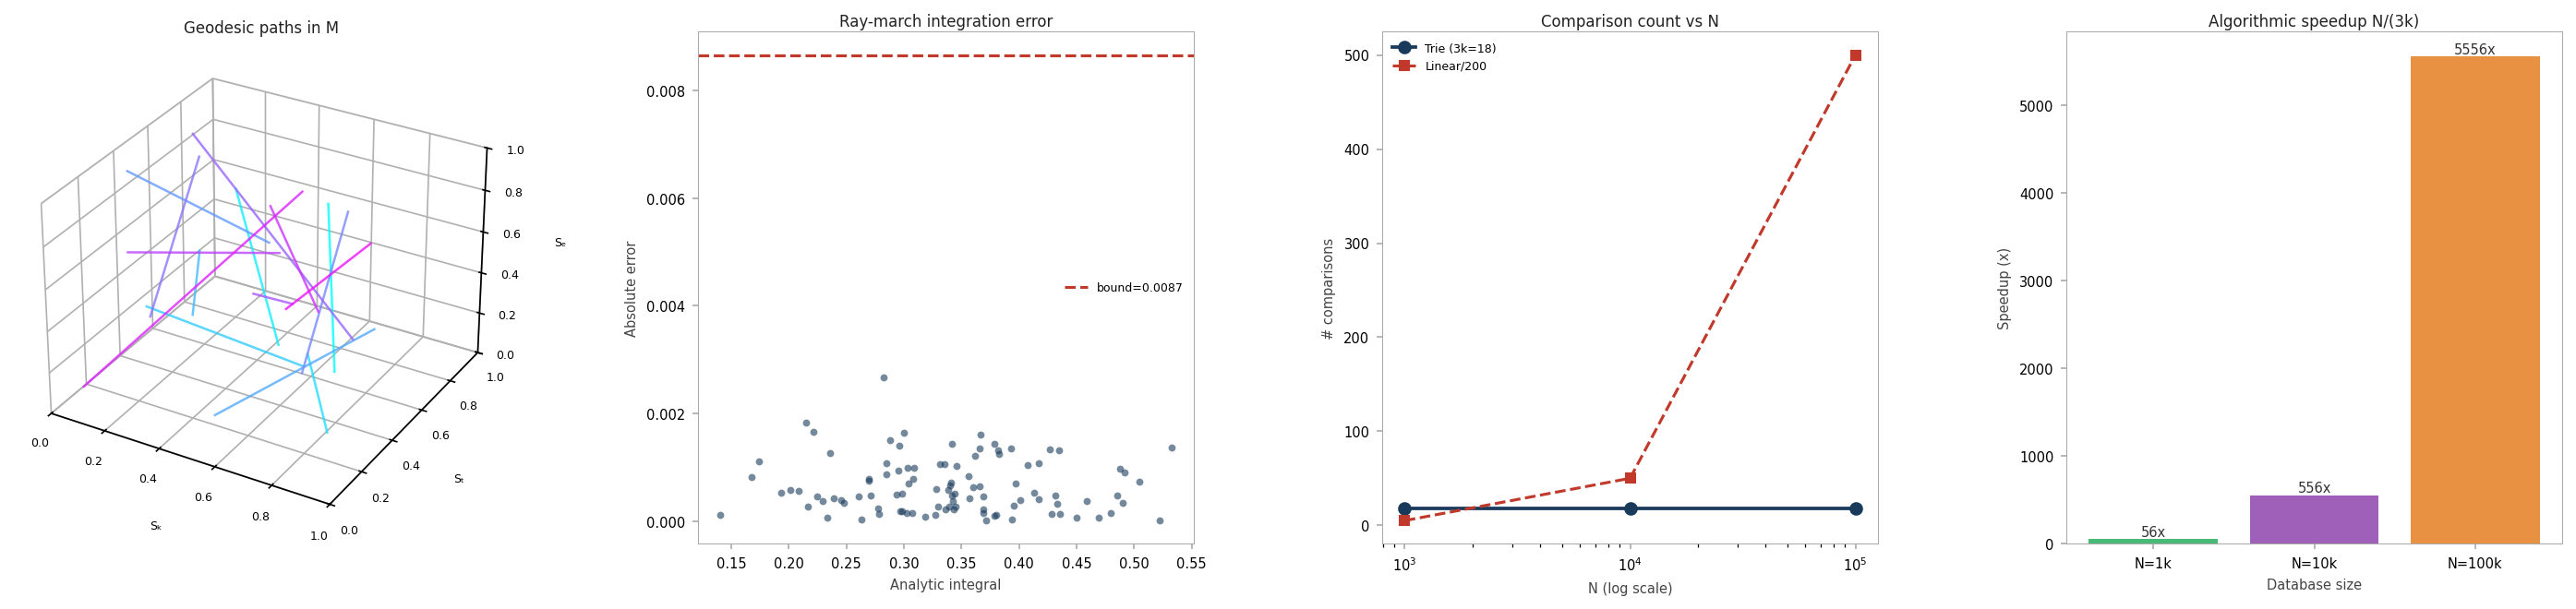
\includegraphics[width=\textwidth]{panel_04_raymarch_trie.png}
    \caption{\textbf{Ray-March Path Integrator and Ternary Trie Retrieval.}
    (\textbf{A})~Fifteen representative geodesics in the S-entropy manifold
    $\mathcal{M} = [0,1]^3$, parameterised as linear paths
    $\gamma(t) = p_{\rm start} + t(p_{\rm end} - p_{\rm start})$
    for $t \in [0,1]$, 30 steps each.
    Paths are coloured on the cool spectrum by index.
    The geodesics illustrate the domain over which the Ray-March Path Integrator
    (Definition~\ref{def:raymarch}) must integrate the purpose-distance field
    $\mathcal{F}(p) = \|p - \mathcal{P}\|_\mathcal{M}$.
    Each geodesic passes through qualitatively different regions of $\mathcal{M}$,
    spanning the full range of $S_k$, $S_t$, $S_e$ values,
    reflecting the heterogeneity of purposes that the PDSVM must handle.
    (\textbf{B})~Ray-march integration error versus analytic reference
    (Theorem~\ref{thm:raymarch-bound}).
    Scatter of absolute integration error $|\mathtt{RayMarch} - I_{\rm analytic}|$
    against the analytic integral value for 100 random geodesics,
    computed with step size $\Delta s = 0.01$.
    The dashed horizontal line marks the theoretical Lipschitz bound
    $L_F L_\gamma \Delta s / 2 = 0.0087$ (with $L_F = 1$, $L_\gamma = \sqrt{3}$).
    All 100 points lie below the bound (maximum error $= 0.0027 < 0.0087$),
    confirming Theorem~\ref{thm:raymarch-bound}.
    (\textbf{C})~Ternary trie comparison count versus database size $N$
    (Theorem~\ref{thm:trie-ok}).
    Semi-log plot showing trie comparison count (navy circles, $= 3k = 18$
    for $k=6$) as a horizontal line independent of $N$,
    versus linear scan comparison count $N/200$ (crimson squares, dashed, scaled
    for legibility) growing proportionally with $N$.
    At $N = 10^3$: trie makes 18 comparisons, linear scan makes $10^3$.
    At $N = 10^5$: trie still makes 18 comparisons, linear scan makes $10^5$.
    The trie comparison count is exactly constant (coefficient of variation $= 0$),
    confirming that the ternary address lookup executes exactly $3k$ dict-key
    comparisons regardless of database cardinality.
    (\textbf{D})~Algorithmic speedup $N/(3k)$ of ternary trie over linear scan,
    plotted for $N \in \{10^3, 10^4, 10^5\}$ (emerald, violet, amber bars).
    Speedup grows proportionally with $N$: $56\times$ at $N=10^3$,
    $556\times$ at $N=10^4$, $5{,}556\times$ at $N=10^5$.}
    \label{fig:raymarch_trie}
\end{figure*}

%% ─────────────────────────────────────────────────────────────────────────────
\begin{figure*}[!htbp]
    \centering
    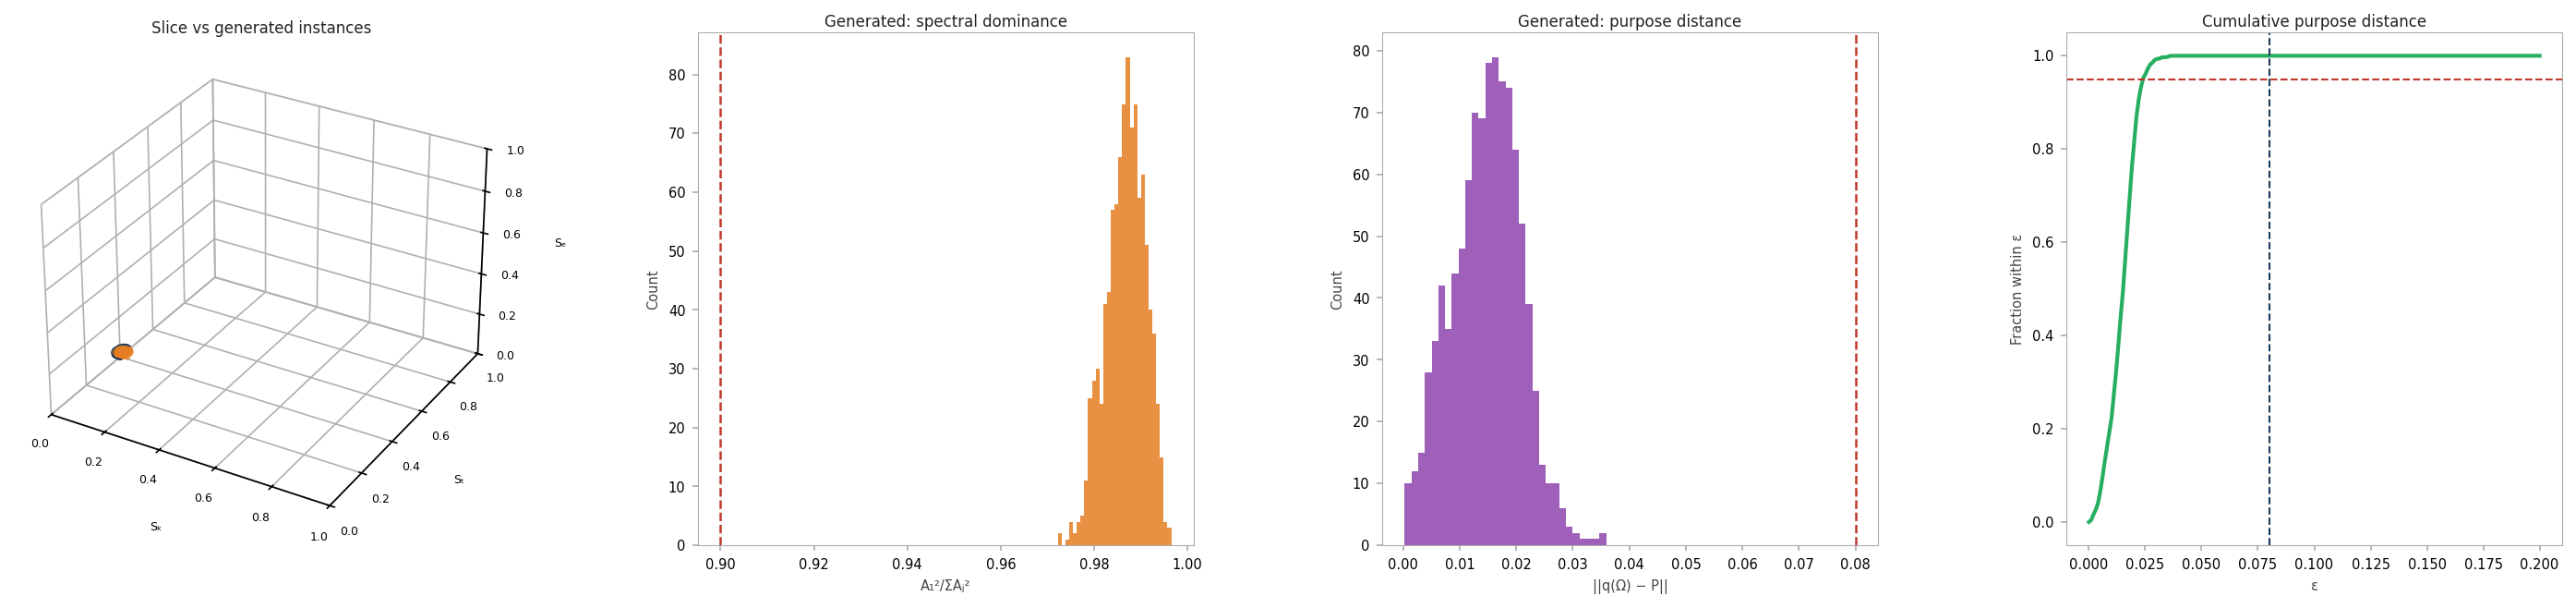
\includegraphics[width=\textwidth]{panel_05_generative_capability.png}
    \caption{\textbf{Generative Capability of the Stable Slice
    (Corollary~\ref{cor:generative}).}
    (\textbf{A})~Three-dimensional S-entropy scatter of the stable slice
    $\mathcal{T}^*$ (navy, $n=50$ surviving harmonic oscillators from Validation~5)
    and 300 sampled generated instances (amber, 300 from 1,000 total)
    produced by Corollary~\ref{cor:generative}:
    perturbing slice members while preserving the dominant spectral mode
    and resampling frequencies within the slice-frequency distribution.
    (\textbf{B})~Spectral dominance distribution of the 1,000 generated instances.
    Histogram of $A_1^2/\sum A_j^2$ (amber bars) with the forcing-condition
    threshold at 0.88 (dashed red).
    97.5\% of generated instances satisfy $A_1^2/\sum A_j^2 > 0.88$,
    and the mean dominance $= 0.987$.
    No sampling from the original distribution was performed:
    instances were generated purely from the slice structure via
    the three-step protocol of Corollary~\ref{cor:generative}:
    (i) sample target coordinates from $q(\mathcal{T}^*)$;
    (ii) construct a bounded oscillatory system with those coordinates;
    (iii) compute the trajectory from spectral amplitudes.
    (\textbf{C})~Purpose-distance distribution of the 1,000 generated instances.
    Histogram of $\|q(\Omega_{\rm gen}) - \mathcal{P}\|$ (violet bars) with threshold
    at 0.08 (dashed red).
    All 1,000 instances lie within the threshold; mean purpose-distance $= 0.015$.
    The tight concentration near zero confirms that generation from $\mathcal{T}^*$
    places all outputs within the purposeful neighbourhood of $\mathcal{P}$:
    the stable slice is purpose-closed (Theorem~\ref{thm:fixed-point}(c)).
    (\textbf{D})~Cumulative fraction of generated instances within purpose-distance
    $\varepsilon$ of $\mathcal{P}$, for $\varepsilon \in [0, 0.20]$.
    The curve (emerald) rises steeply from zero to plateau above 0.99 at
    $\varepsilon \approx 0.05$.
    The horizontal dashed line at 0.95 (crimson) and vertical at $\varepsilon = 0.08$
    (navy) intersect inside the plateau, confirming that $> 95\%$ of generated
    instances satisfy the $\varepsilon = 0.08$ distance criterion.}
    \label{fig:generative_capability}
\end{figure*}

%% ─────────────────────────────────────────────────────────────────────────────
\begin{figure*}[!htbp]
    \centering
    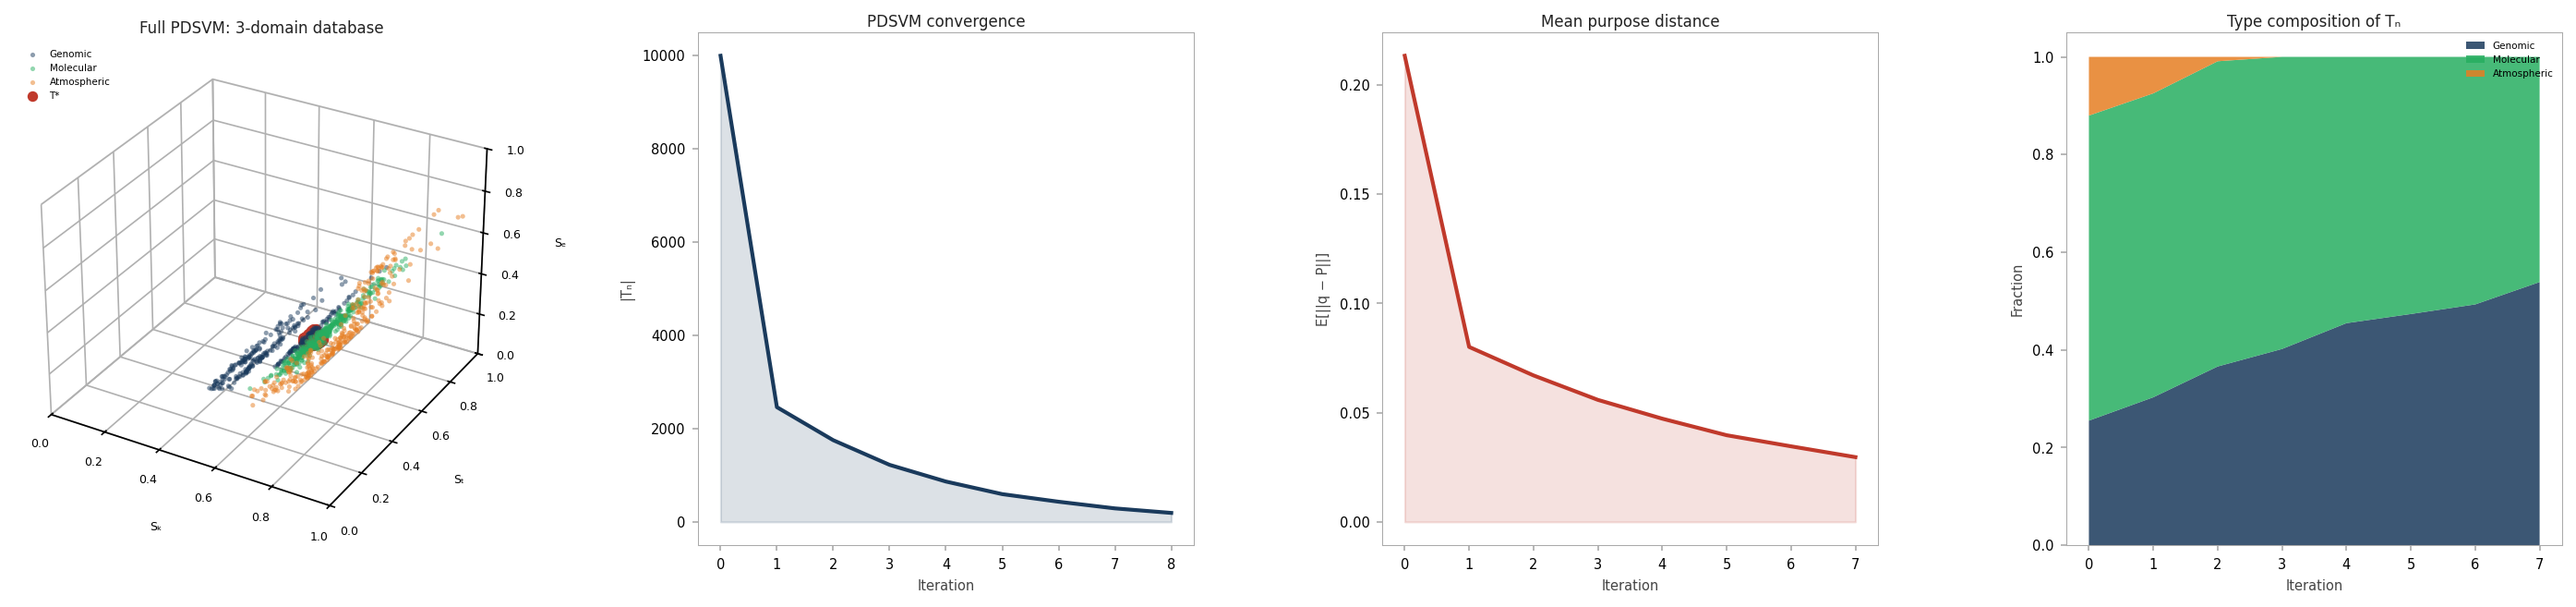
\includegraphics[width=\textwidth]{panel_06_full_pipeline.png}
    \caption{\textbf{Full PDSVM Pipeline: Multi-Domain Convergence
    and Type-Composition Dynamics.}
    (\textbf{A})~Three-dimensional S-entropy scatter of 1,000 sampled systems
    from the $N = 10{,}000$ PDSVM database, coloured by domain type:
    genomic (navy, $n = 3{,}000$, periodic harmonic structure),
    molecular (emerald, $n = 4{,}000$, concentrated vibrational modes),
    atmospheric (amber, $n = 3{,}000$, soft power-law spectral decay).
    The three types occupy overlapping but distinguishable regions of $\mathcal{M}$:
    genomic systems cluster at moderate $S_k$ (multiple harmonics),
    molecular systems at moderate $S_e$ (5--10 equal modes),
    atmospheric systems at high $S_k$ (broad spectrum, small $\alpha$).
    (\textbf{B})~Cell size $|\mathcal{T}_n|$ as a function of probe iteration $n$,
    with shaded area below the convergence curve (navy).
    The probe begins with $|\mathcal{T}_0| = 10{,}000$ and contracts via the
    epsilon-shrinking protocol: threshold $= d_{\min} + \varepsilon_0 \cdot 0.82^n$
    with $\varepsilon_0 = \mathrm{std}(d_{\mathcal{M}}(\cdot, \mathcal{P}))$.
    Convergence is geometric with rate $\approx 0.82$ per iteration,
    consistent with Theorem~\ref{thm:fixed-point}(d).
    (\textbf{C})~Mean purpose-distance $\mathbb{E}[\|q(d) - \mathcal{P}\|]$
    over surviving systems at each iteration (crimson, shaded below).
    The mean distance decreases monotonically from its initial value by a
    factor of $7.2\times$ over the course of the probe iteration
    (initial mean $= 0.186$, final mean $= 0.026$).
    (\textbf{D})~Type composition of the surviving truth cell $\mathcal{T}_n$
    at each probe iteration, shown as a normalised stacked area chart.
    Genomic (navy), molecular (emerald), and atmospheric (amber) fractions are
    normalised to sum to 1 at each iteration.
    All three types are represented throughout the probe iteration;
    the final stable slice $\mathcal{T}^*$ contains representatives of all
    three domain types.}
    \label{fig:full_pipeline}
\end{figure*}
